% vim:ft=tex:
%
\documentclass[letterpaper, 12pt]{article}
\usepackage[utf8]{inputenc}
\usepackage[twoside, margin=0.8in]{geometry}
\usepackage[bookmarks=true, hidelinks, pagebackref=true, linktoc=all]{hyperref}
\usepackage{setspace}
\usepackage{float}
\usepackage{booktabs}
\usepackage{amsmath}
\usepackage{amssymb}
\usepackage{graphicx}
\usepackage{fancyhdr}
\usepackage{enumitem}
\usepackage{listings}

\linespread{1.6}

\pagestyle{fancy}
\fancyhf{}
\rhead{Warm Up Project}
\lhead{COMP353}
\rfoot{\thepage}

\title{
  \textsc{\huge A Simple Database for a Financial Institution}\\
  Warm-up Project
  \vspace*{4em}
}
\author{
  Group ID: \textbf{td\_comp353\_2}\\\\
  Yassin BAH 40077524\\
  Joel Dusablon SENECAL 40035704\\
  Feng ZHAO 40021856\\
  Alireza SARI 40032394\\ 
  %Presented to \\
  %\textsc{Dr. Khaled Jababo}
  \vspace*{6em}
}

\begin{document}
\maketitle
\newpage


\section{Database Design}
\subsection{Assumptions}
In developping and designing this database, certain assumptions have been made.
The goal of this section is to list them in order to help clarify why the database is created the way it is.

\subsubsection{Branch}
A branch has a unique ID that allows for the distinction of if multiple branches are in the same area.
A branch needs to have one manager at all times.
In relational terms, it means the attribute cannont be null in the Branch table.
All the branches of the bank, including the head office, should be in this table.
The head office is denoted by a flag that is set to 1 for the record of the head office.
Furthermore, the manager of the head office represents the president of the bank.
Following this assumption, the president of the bank is also an employee and has an equivalent entry in the Employee table.
Moreover, it was assumed that the address of the branch as well as its opening date must contain a value (i.e. they cannot be null), while the phone and fax number can initially be void.   

\subsubsection{Employee}
Every employee has a unique identifier.
Basic assumptions about employees are that each record must have their first name, last name, starting date and a branch ID that cannot be null at the onset.
Employee only works at one branch and that branch has to be open.
That means that the branch ID for in the Employee table cannot be null at any time.
However, the email and phone fields for a particular employee can hold null values, whereas the salary, while not nullable, can still hold a default value of 0. 
%An employee can only hold one position (ex. the president of the company is not the manager of the head office).
All service general managers work at the head office.
In order to know the general manager of each service, the Service table needs to be looked up.

\subsubsection{Client}
Clients also have unique identifier.
Like employees, clients have a first name, a last name and a branch attributes that cannot be null.
A client needs to be associated with one branch at all times.

\subsubsection{Account}
Accounts belong to a specific client and may not be shared.
Clients, however, may have multiple accounts linked to them.
An account has to be associated with a current client of the bank.
An account can only have one option associated with it. %, which could be for a US account
Credit limits are associated with accounts rather than clients.
Reason being is that a client may have a business account and a personal account, but the credit limit for either account might be different.
A similar situation occurs with the interest rate, they can vary depending on multiple factors and may hold a range of values.

%\subsubsection{Interest Rate}
%%This table gives the default interest rate for the bank when looking at each combination of service and the account type. 
%Interest rates vary by account, it may be the default value that the bank has set but may also be different based on some negotiations with the bank.
%For example, the interest rate for a checking account is 0\% by default.
%Therefore the interest rate table gives the default values for the percentage that the bank has set regarding the different combinations of services and type of accounts.

\subsubsection{Services}
As stated previously, the services contain a list of services that the bank offers as well as the ID of the general manager for said service.
Therefore, the value of the manager id cannot be null. All general managers are thus also considered employees.

%\subsubsection{Charge Plan}
%Charge plans \ldots

\newpage
\subsection{E/R Diagram}

\begin{figure}[H]
  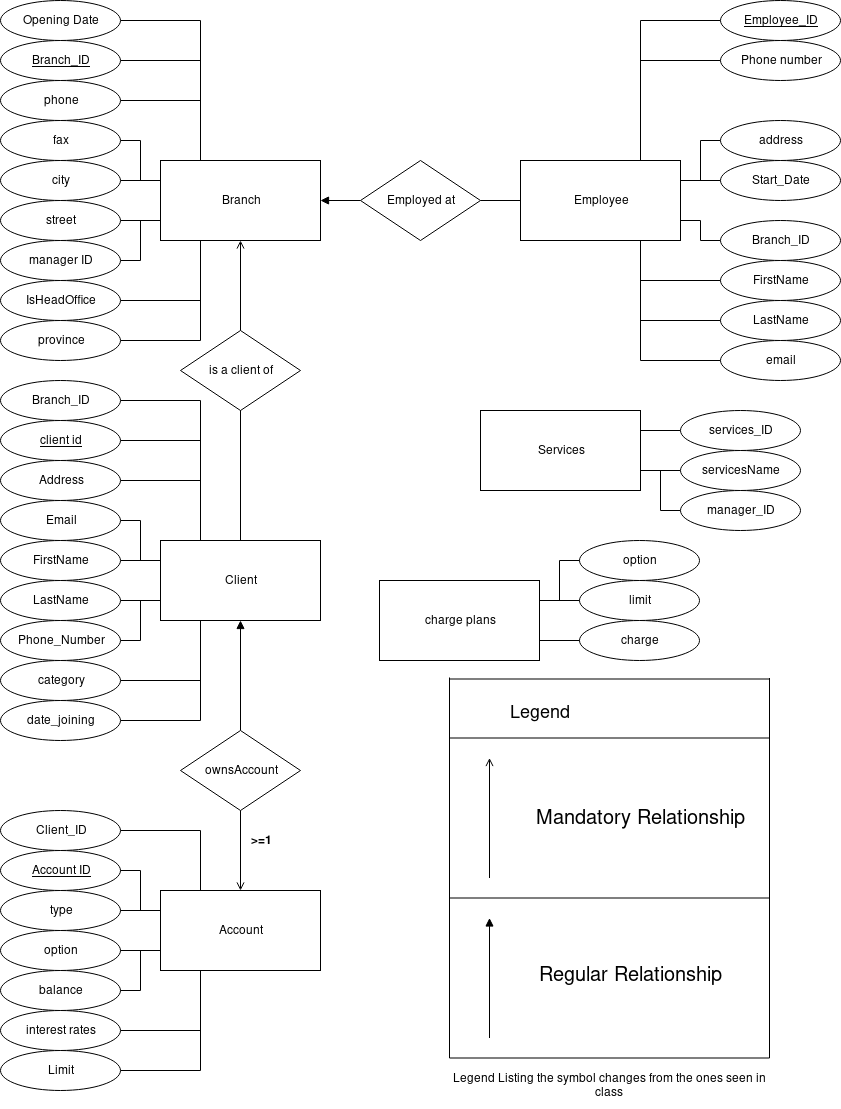
\includegraphics[scale=0.55]{images/DB_WARMUP.png}
\end{figure}

\newpage
\section{Schema}

\begin{lstlisting}[language=sql]
/* Employee */
CREATE TABLE IF NOT EXISTS Employee (
        employee_id     int not null auto_increment,
        firstName       varchar(255) not null,
        lastName        varchar(255) not null,
        addr            varchar(255),
        start_date      date not null,
        salary          decimal(14,2) default 0,
        email           varchar(255),
        phone           varchar(255),
        branch_id       int,
        primary key(employee_id)
);


/* Branch */
CREATE TABLE IF NOT EXISTS Branch (
        branch_id       int not null auto_increment,
        province        varchar(255) not null,
        city            varchar(255) not null,
        street          varchar(255) not null,
        phone           varchar(255),
        fax             varchar(255),
        opening_date    date not null,
        manager_id      int ,
        isHeadOffice    tinyint(1),
        FOREIGN KEY (manager_id) REFERENCES Employee(employee_id),
        primary key(branch_id)
);

ALTER TABLE Employee ADD FOREIGN KEY (branch_id) 
	REFERENCES Branch(branch_id);


/* Client */
CREATE TABLE IF NOT EXISTS Client (
        client_id       int not null auto_increment,
        firstName       varchar(255) not null,
        lastName        varchar(255) not null,
        addr            varchar(255) not null,
        dob             date not null,
        joining_date    date not null,
        email           varchar(255),
        phone           varchar(255),
        category        varchar(255) default 'Regular',
        branch_id       int not null,
        foreign key(branch_id) references Branch(branch_id),
        primary key(client_id)
);

/* Account */
CREATE TABLE IF NOT EXISTS Account (
        account_id      int not null auto_increment,
        client_id       int not null,
        account_type    varchar(255) not null,
        account_option  varchar(255) not null,
        balance         decimal(14,2),
        credit_limit    decimal(14,2),
        interest_rate   float,
        foreign key(client_id) references Client(client_id),
        primary key(account_id)
);

/* Services */
CREATE TABLE IF NOT EXISTS Services (
        service_id      int not null auto_increment,
        service_name    char(50),
        manager_id      int not null,
        foreign key(manager_id) references Employee(employee_id),
        primary key(service_id)
);

/* Charge plans */
CREATE TABLE IF NOT EXISTS ChargePlan (
        charge_id       int not null,
        draw_limit      float,
        charge_value    float,
        primary key(charge_id)
);

\end{lstlisting}

\newpage
\section{Queries}

\begin{enumerate}[label=\arabic*.]
  \item All of the tables
    \begin{lstlisting}[language=sql]
SHOW tables;
  \end{lstlisting}
\begin{figure}[H]
  \centering
  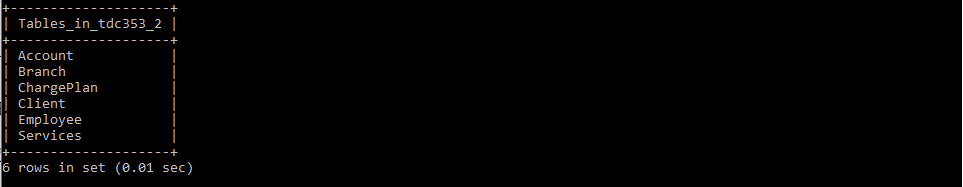
\includegraphics[scale=0.6]{images/Query_1.PNG}
  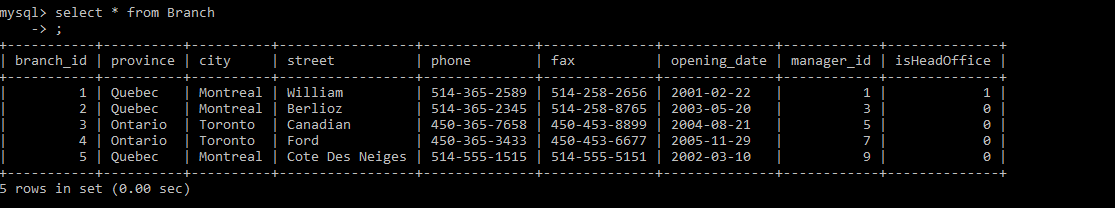
\includegraphics[scale=0.5]{images/Query_1_1.PNG}
  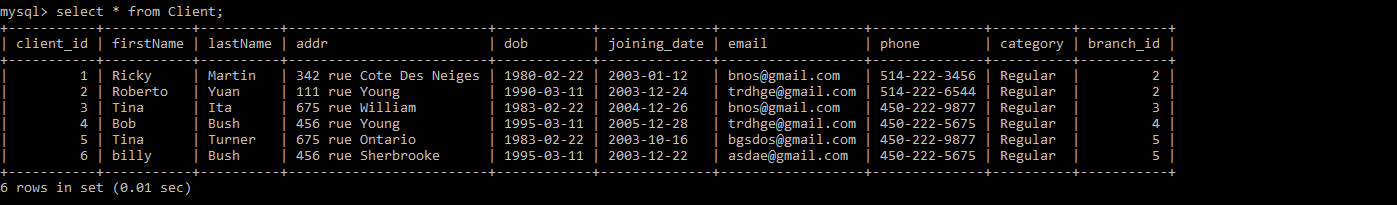
\includegraphics[scale=0.5]{images/Query_1_2.PNG}
  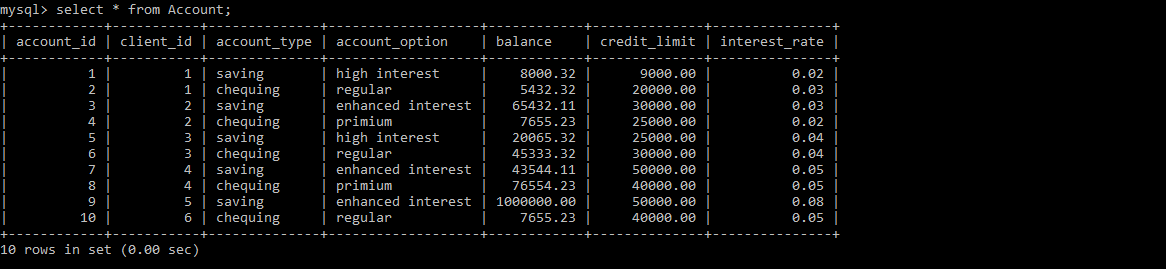
\includegraphics[scale=0.5]{images/Query_1_3.PNG}
  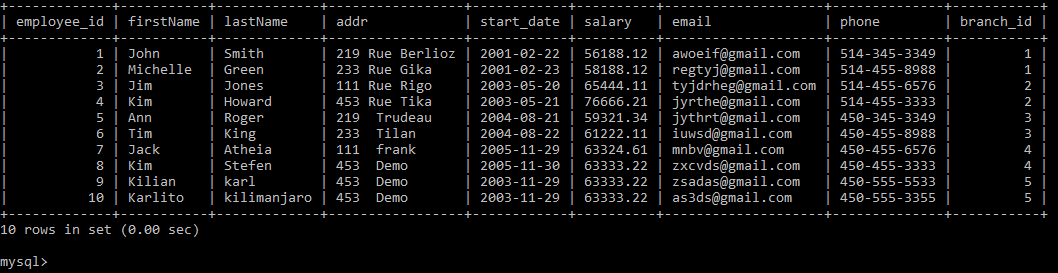
\includegraphics[scale=0.5]{images/Query_1_5.PNG}
  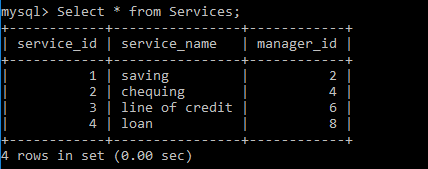
\includegraphics[scale=0.6]{images/Query_1_4.PNG}
\end{figure}
  \item List of all the branches grouped by city and ordered by oldest branch.
    \begin{lstlisting}[language=sql]
SELECT * FROM Branch ORDER BY city ASC, opening_date ASC;
  \end{lstlisting}
\begin{figure}[H]
  \centering
  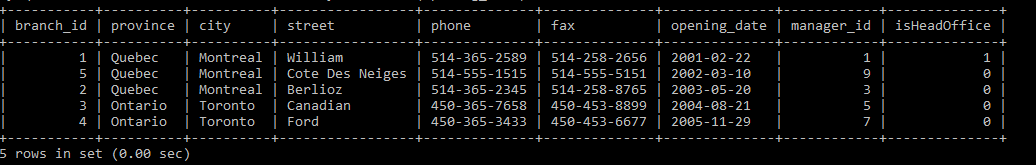
\includegraphics[scale=0.6]{images/Query_2.PNG}
\end{figure}
  \item List of all clients with DOB between 1990 and 2017.
    \begin{lstlisting}[language=sql]
SELECT client_id, dob FROM Client WHERE 
	DATE(dob) > '1990-01-01' AND DATE(dob) < '2018-01-01';
  \end{lstlisting}
\begin{figure}[H]
  \centering
  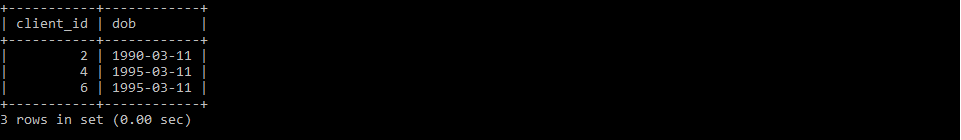
\includegraphics[scale=0.6]{images/Query_3.PNG}
\end{figure}
  \item List all clients of a branch who has either a checking or savings account of balance more than CND 10,000.00.
    \begin{lstlisting}[language=sql]
SELECT c.firstName, c.lastName, a.balance FROM Client c,
	Account a WHERE a.balance >= 10000.00 AND 
	a.account_type = 'saving' AND a.client_id = c.client_id
	AND c.branch_id = 3;
  \end{lstlisting}
\begin{figure}[H]
  \centering
  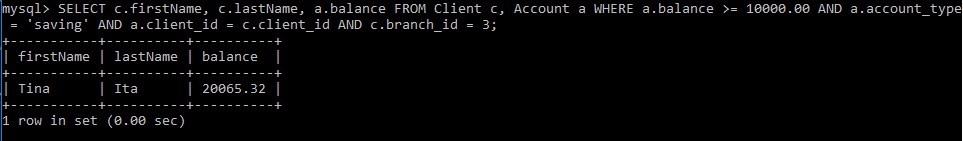
\includegraphics[scale=0.6]{images/Query_4.PNG}
\end{figure}
  \item List of all clients of a branch who has a line of credit of limit CND 25,000.00 with an interest rate of 7.5\% or below.
    \begin{lstlisting}[language=sql]
SELECT c.firstName, c.lastName, a.credit_limit, a.interest_rate 
	FROM Client c, Account a WHERE a.credit_limit = 25000.00
	AND a.interest_rate <= 0.075 AND a.client_id = c.client_id 
	AND c.branch_id = 2;
  \end{lstlisting}
\begin{figure}[H]
  \centering
  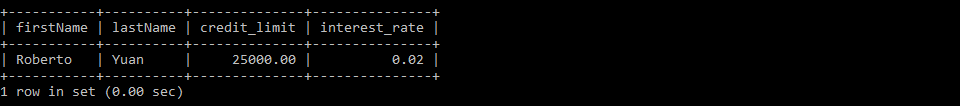
\includegraphics[scale=0.6]{images/Query_5.PNG}
\end{figure}
  \item List details of a client named Roberto.
    \begin{lstlisting}[language=sql]
SELECT * FROM Client WHERE 
	firstName = 'Roberto' OR lastName = 'Roberto';
  \end{lstlisting}
\begin{figure}[H]
  \centering
  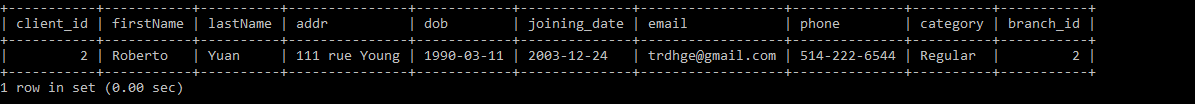
\includegraphics[scale=0.6]{images/Query_6.PNG}
\end{figure}
  \item List of all clients of 'Cote Des Neiges' branch.
    \begin{lstlisting}[language=sql]
SELECT client_id FROM Client WHERE branch_id IN (
	SELECT branch_id FROM Branch WHERE street LIKE
	'%Cote Des Neiges%');
  \end{lstlisting}
\begin{figure}[H]
  \centering
  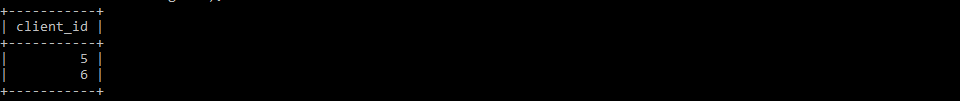
\includegraphics[scale=0.6]{images/Query_7.PNG}
\end{figure}
  \item List of clients who have at least 1,000,000 CDN dollar in their savings account.
    \begin{lstlisting}[language=sql]
SELECT DISTINCT client_id FROM Account WHERE 
	account_type = 'saving' AND balance >= 1000000;
  \end{lstlisting}
\begin{figure}[H]
  \centering
  
\includegraphics[scale=0.6]{images/Query_8.PNG}
\end{figure}
  \item List of all the services along with the general manager for each service.
    \begin{lstlisting}[language=sql]
SELECT s.service_name, e.firstName, e.lastName 
	FROM Services s, Employee e WHERE s.manager_id = e.employee_id;
  \end{lstlisting}
\begin{figure}[H]
  \centering
  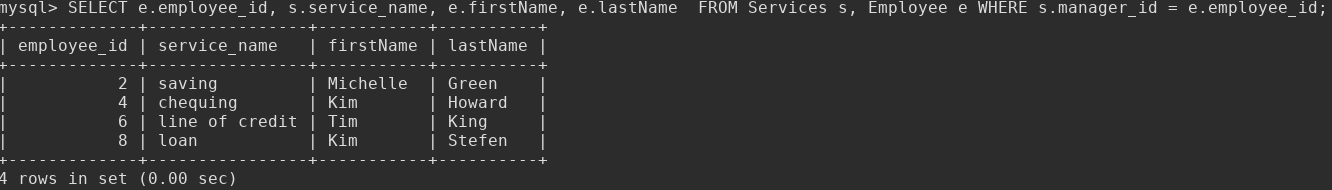
\includegraphics[scale=0.6]{images/Query_9.PNG}
\end{figure}
  \item Complete details of the president of the bank.
    \begin{lstlisting}[language=sql]
SELECT * FROM Employee WHERE employee_id = (
	SELECT manager_id FROM Branch WHERE isHeadOffice = 1);
  \end{lstlisting}
\begin{figure}[H]
  \centering
  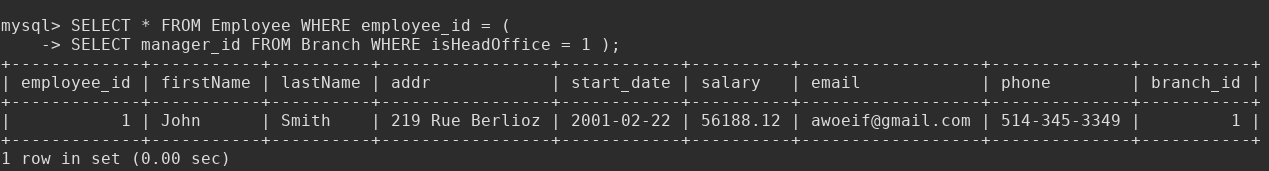
\includegraphics[scale=0.45]{images/query_10.png}
\end{figure}

\end{enumerate}


\end{document}
